% Diagrams of an OpenCog agent in a virtual world
% Ben Goertzel, Cosmo Harrigan

\documentclass{article}
\usepackage{tikz}
\usepackage{hieroglf}
\usepackage[margin=20pt]{geometry}
\usetikzlibrary{chains,patterns,shadows,fit,backgrounds,positioning,calc,arrows.meta}

\begin{document}

% Figure 1
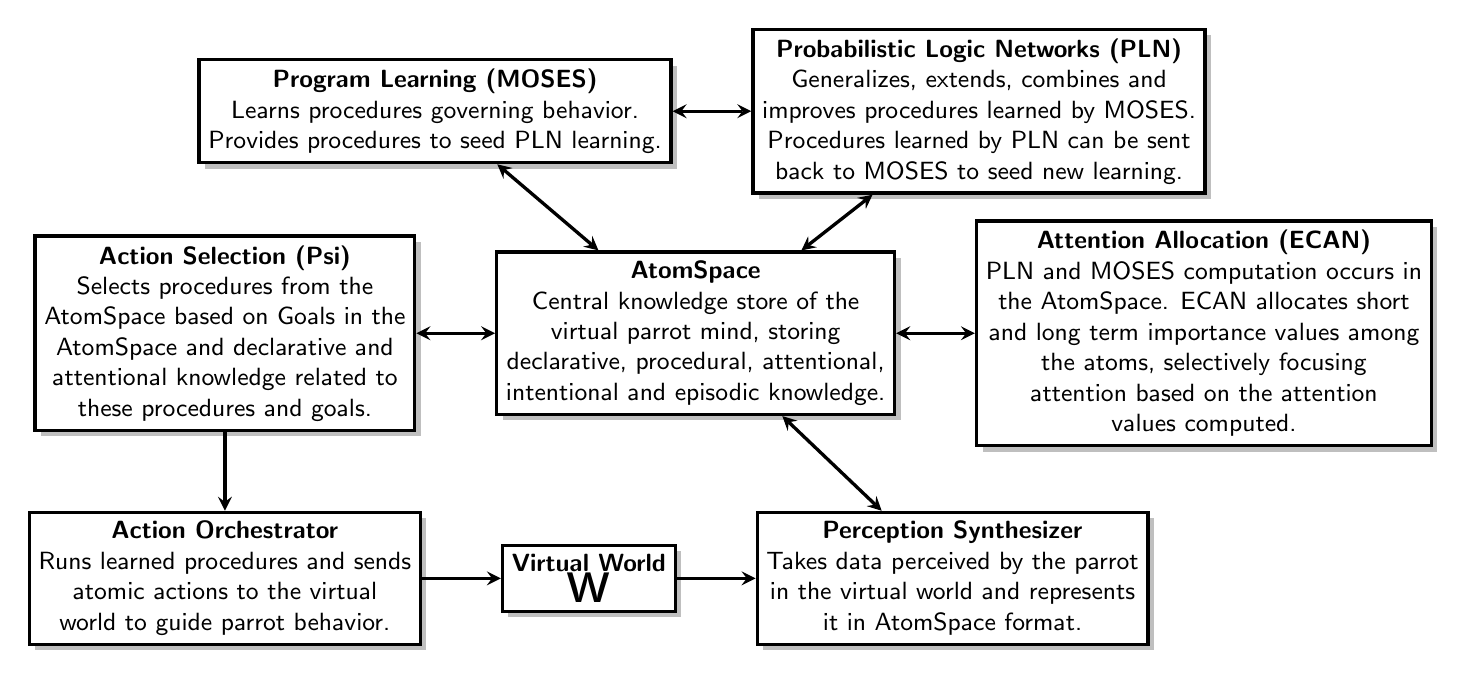
\begin{tikzpicture}
    [font=\small\sffamily, very thick]
    
    % AtomSpace
    \node (atomspace) [draw, align=center, drop shadow, fill=white]
    {
    \textbf{AtomSpace} \\
    Central knowledge store of the\\
    virtual parrot mind,  storing\\
    declarative, procedural, attentional,\\
    intentional and episodic knowledge.
    };
    
    % ECAN
    \node (ecan) [draw, align=center, drop shadow, fill=white, right = 1cm of atomspace.east]
    {
    \textbf{Attention Allocation (ECAN)} \\
    PLN and MOSES computation occurs in\\
    the AtomSpace. ECAN allocates short\\
    and long term importance values among\\
    the atoms, selectively focusing\\
    attention based on the attention\\
    values computed.
    };
    
    % Psi
    \node (psi) [draw, align=center, drop shadow, fill=white, left = 1cm of atomspace.west]
    {
    \textbf{Action Selection (Psi)} \\
    Selects procedures from the\\
    AtomSpace based on Goals in the\\
    AtomSpace and declarative and\\
    attentional knowledge related to\\
    these procedures and goals.
    };
    
    % PLN
    \node (pln) [draw, align=center, drop shadow, fill=white, above right = 1cm of atomspace.north]
    {
    \textbf{Probabilistic Logic Networks (PLN)} \\
    Generalizes, extends, combines and\\
    improves procedures learned by MOSES.\\
    Procedures learned by PLN can be sent\\
    back to MOSES to seed new learning.
    };
    
    % MOSES
    \node (moses) [draw, align=center, drop shadow, fill=white, left = 1cm of pln.west]
    {
    \textbf{Program Learning (MOSES)} \\
    Learns procedures governing behavior.\\
    Provides procedures to seed PLN learning.
    };
    
    % Action Orchestrator
    \node (action) [draw, align=center, drop shadow, fill=white, below = 1cm of psi]
    {
    \textbf{Action Orchestrator} \\
    Runs learned procedures and sends\\
    atomic actions to the virtual\\
    world to guide parrot behavior.
    };
    
    % Virtual World
    \node (virtual-world) [draw, align=center, drop shadow, fill=white, right = 1cm of action]
    {
    \textbf{Virtual World} \\
    \Huge{\textpmhg{w}}
    };
    
    % Perception Synthesizer
    \node (perception) [draw, align=center, drop shadow, fill=white, right = 1cm of virtual-world]
    {
    \textbf{Perception Synthesizer} \\
    Takes data perceived by the parrot\\
    in the virtual world and represents\\
    it in AtomSpace format.
    };
    
    % Draw edges between boxes
    \draw
    [stealth-stealth] (atomspace) edge (ecan)
    [stealth-stealth] (atomspace) edge (psi)
    [stealth-stealth] (atomspace) edge (pln)
    [stealth-stealth] (atomspace) edge (moses)
    [stealth-stealth] (moses) edge (pln)
    [stealth-stealth] (perception) edge (atomspace)
    [-stealth] (virtual-world) edge (perception)
    [-stealth] (action) edge (virtual-world)
    [-stealth] (psi) edge (action)
    ;
    
\end{tikzpicture}

\hfill\break
\hfill\break

% Figure 2
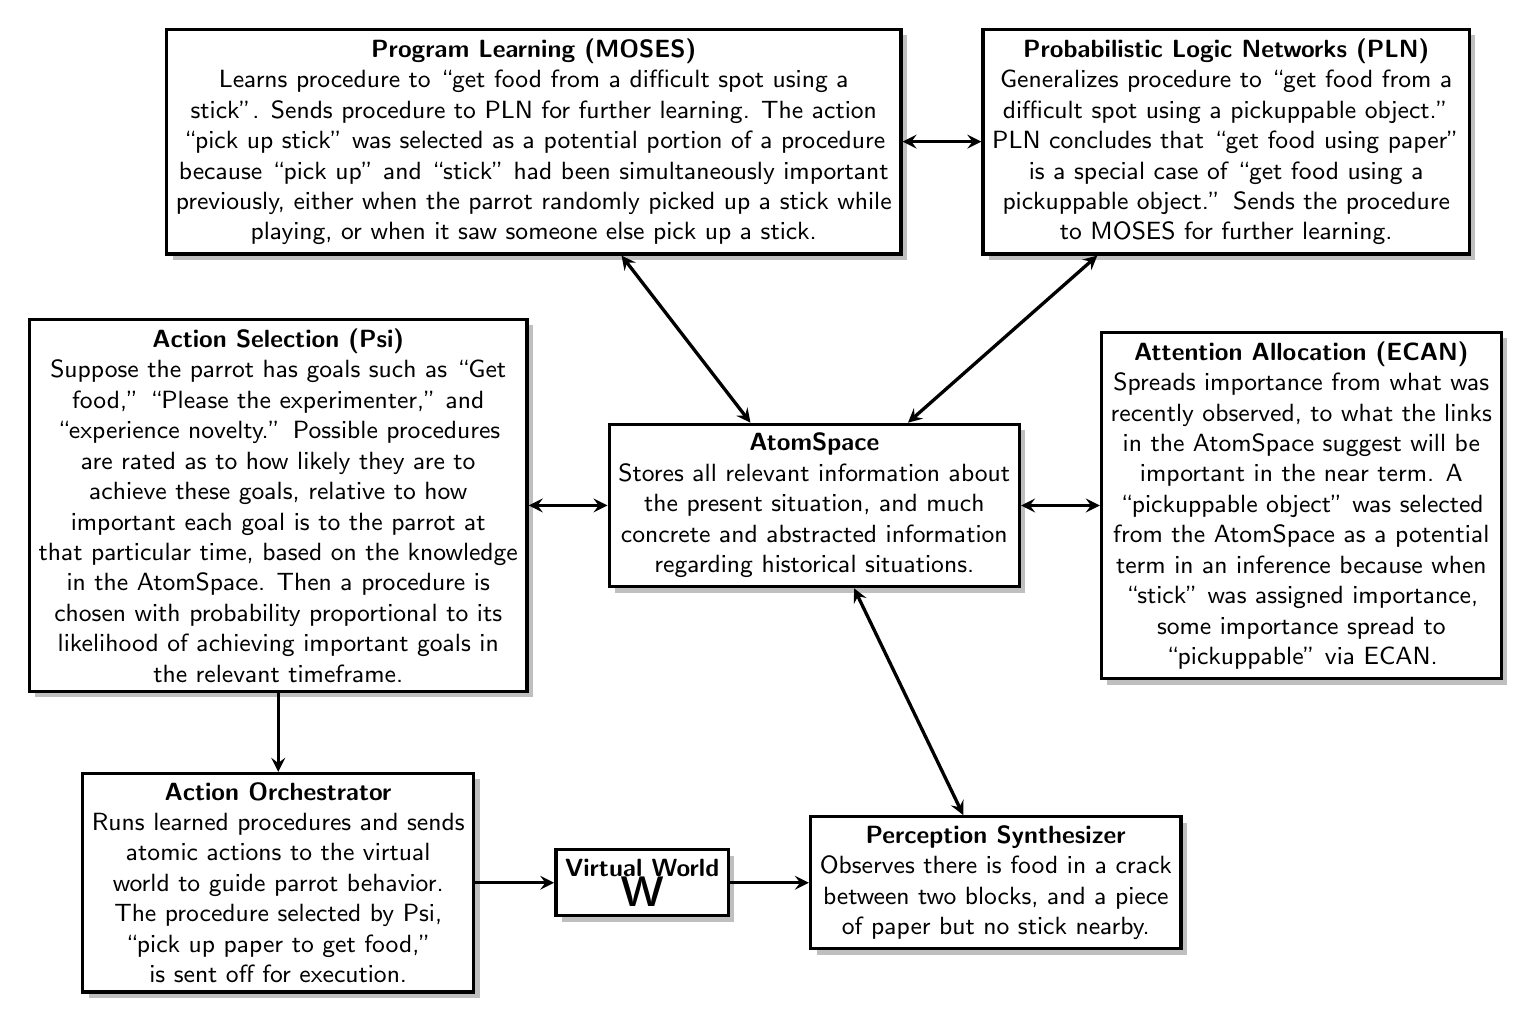
\begin{tikzpicture}
    [font=\small\sffamily, very thick]
    
    % AtomSpace
    \node (atomspace) [draw, align=center, drop shadow, fill=white]
    {
    \textbf{AtomSpace} \\
    Stores all relevant information about\\
    the present situation, and much\\
    concrete and abstracted information\\
    regarding historical situations.
    };
    
    % ECAN
    \node (ecan) [draw, align=center, drop shadow, fill=white, right = 1cm of atomspace.east]
    {
    \textbf{Attention Allocation (ECAN)} \\
    Spreads importance from what was\\
    recently observed, to what the links\\
    in the AtomSpace suggest will be\\
    important in the near term. A\\
    ``pickuppable object'' was selected\\
    from the AtomSpace as a potential\\
    term in an inference because when\\
    ``stick'' was assigned importance,\\
    some importance spread to\\
    ``pickuppable'' via ECAN.
    };
    
    % Psi
    \node (psi) [draw, align=center, drop shadow, fill=white, left = 1cm of atomspace.west]
    {
    \textbf{Action Selection (Psi)} \\
    Suppose the parrot has goals such as ``Get\\
    food,'' ``Please the experimenter,'' and\\
    ``experience novelty.'' Possible procedures\\
    are rated as to how likely they are to\\
    achieve these goals, relative to how\\
    important each goal is to the parrot at\\
    that particular time, based on the knowledge\\
    in the AtomSpace. Then a procedure is\\
    chosen with probability proportional to its\\
    likelihood of achieving important goals in\\
    the relevant timeframe.
    };
    
    % PLN
    \node (pln) [draw, align=center, drop shadow, fill=white, above right = 3cm of atomspace.north]
    {
    \textbf{Probabilistic Logic Networks (PLN)} \\
    Generalizes procedure to ``get food from a\\
    difficult spot using a pickuppable object.''\\
    PLN concludes that ``get food using paper''\\
    is a special case of ``get food using a\\
    pickuppable object.'' Sends the procedure\\
    to MOSES for further learning.
    };
    
    % MOSES
    \node (moses) [draw, align=center, drop shadow, fill=white, left = 1cm of pln.west]
    {
    \textbf{Program Learning (MOSES)} \\
    Learns procedure to ``get food from a difficult spot using a\\
    stick''. Sends procedure to PLN for further learning. The action\\
    ``pick up stick'' was selected as a potential portion of a procedure\\
    because ``pick up'' and ``stick'' had been simultaneously important\\
    previously, either when the parrot randomly picked up a stick while\\
    playing, or when it saw someone else pick up a stick.
    };
    
    % Action Orchestrator
    \node (action) [draw, align=center, drop shadow, fill=white, below = 1cm of psi]
    {
    \textbf{Action Orchestrator} \\
    Runs learned procedures and sends\\
    atomic actions to the virtual\\
    world to guide parrot behavior.\\
    The procedure selected by Psi,\\
    ``pick up paper to get food,''\\
    is sent off for execution.
    };
    
    % Virtual World
    \node (virtual-world) [draw, align=center, drop shadow, fill=white, right = 1cm of action]
    {
    \textbf{Virtual World} \\
    \Huge{\textpmhg{w}}
    };
    
    % Perception Synthesizer
    \node (perception) [draw, align=center, drop shadow, fill=white, right = 1cm of virtual-world]
    {
    \textbf{Perception Synthesizer} \\
    Observes there is food in a crack\\
    between two blocks, and a piece\\
    of paper but no stick nearby.
    };
    
    % Draw edges between boxes
    \draw
    [stealth-stealth] (atomspace) edge (ecan)
    [stealth-stealth] (atomspace) edge (psi)
    [stealth-stealth] (atomspace) edge (pln)
    [stealth-stealth] (atomspace) edge (moses)
    [stealth-stealth] (moses) edge (pln)
    [stealth-stealth] (perception) edge (atomspace)
    [-stealth] (virtual-world) edge (perception)
    [-stealth] (action) edge (virtual-world)
    [-stealth] (psi) edge (action)
    ;
    
\end{tikzpicture}

\end{document}
